\documentclass{standalone}

\usepackage{tikz}
\usetikzlibrary{angles,quotes}
\usepackage{amsmath,amssymb,amsfonts}

\usepackage{pgfplots}
\definecolor{darkgreen}{rgb}{0.0, 0.42, 0.24}
\definecolor{amethyst}{rgb}{0.6, 0.4, 0.8}

\pgfplotsset{compat=newest}
\pgfplotsset{every axis/.append style={
                     tick label style={font=\footnotesize},
                 }}

\usepackage{siunitx}
\DeclareSIUnit \ly {ly}
\usepgfplotslibrary{units}
\begin{document}
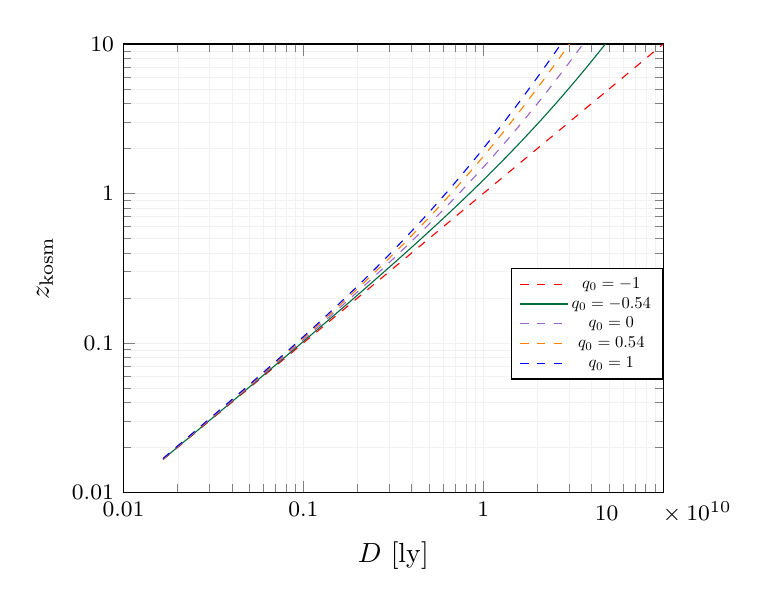
\begin{tikzpicture}
 \begin{axis}[xmin=0.01,xmax=10,ymin=0.01,ymax=10,
 grid=both,
    grid style={line width=.1pt, draw=gray!10},
    major grid style={line width=.2pt,draw=gray!10},
     minor tick num=5,
 xmode=log,
 ymode=log,
 xtick={0.01,0.1,1,10},
 xticklabels={0.01,0.1,1,$10\ \ \ \ \ \times10^{10}$},
 log ticks with fixed point,
 xlabel=$D $,ylabel=$z_{\text{kosm}}$,
 x unit=ly,
legend style={nodes={scale=0.6, transform shape},at={(1,0.5)}}]

 \addplot[color=red,samples=300,dashed]{x+((1-1)/2)*x^2};
     \addplot[color=darkgreen,samples=300]{x+((1-0.54)/2)*x^2};
      \addplot[color=amethyst,samples=300,dashed]{x+((1)/2)*x^2};
       \addplot[color=orange,samples=300,dashed]{x+((1+0.54)/2)*x^2};
        \addplot[color=blue,samples=300,dashed]{x+((1+1)/2)*x^2};

        \addplot[color=red,samples=300, domain=5:10,dashed]{x+((1-1)/2)*x^2};
        
        \addlegendentry{$q_0=-1$};
        \addlegendentry{$q_0=-0.54$};
        \addlegendentry{$q_0=0$};
        \addlegendentry{$q_0=0.54$};
        \addlegendentry{$q_0=1$};
 \end{axis}

\end{tikzpicture}
\end{document}